\chapter{Налаштування та робота із таймерами у контролерах atmega328} 
\label{chapter:first}

\section{Короткі відомості для використовуваних побітових операцій}

Оскільки весь процес роботи із таймерами полягає у використанні реєстрів, нагадаємо деякі побітові операції, що стануть у нагоді.
\begin{itemize}
    \item Побітове \textbf{АБО (x|y)}: Нехай задано число $x = 2$ та $у = 4$. Їхні представлення у двійковій системі: $x= 10$ та $y = 100$. Результатом роботи оператора або буде $x|y = 110$
    \item Функція \textbf{bit(n)}: Створення байту, в якому біт номер $n =1$, а всі інші рівні нулю. Її зручно використовувати в парі із попереднім оператором, коли потрібно в існуючому байті певному біту приписати 1.
\end{itemize}

\section{Принцип роботи таймерів}

Робота таймеру полягає у збільшенні певної змінної, що носить ім'я рахункового регістру. Він збільшує її на один, крок за кроком, аж поки не досягне максимального значення, що повязане із розміром регістру. У момент переповнення таймер встановлює біт відповідного прапорця. 

Ми можемо вручну перевіряти стан цього прапорця, але краще використовувати таймерний перемикач, який викликає переривання автоматично, після встановлення прапорця. Звісно ми можемо привязати підпрограму переривання, в якій написати все, для чого нам власне і потрібен таймер.

\section{Типи таймерів, доступні для arduino uno \cite{habr}}
% Для плати arduino Uno, на відміну від arduino Mega, доступні лише три таймера \cite{habr}:
\begin{itemize}
\item \textbf{Timer0}: 8-бітний таймер (максимальне значення 255), який використовується стандартними функціями delay() та millis(). Тому краще не використовувати цей таймер без потреби.
\item \textbf{Timer1}: 16-бітний таймер (максимальне значення 65535), який використовується бібліотекою Arduino Servo.
\item \textbf{Timer2}: 8-бітний таймер, який використовується функцією tone().
\end{itemize}

\section{Конфігурація регістрів}

Для налаштування роботи таймеру використовується 2 регістри: TCCRxA та TCCRxB, де х - номер таймеру. Кожен з них містить 8 біт. \cite{datasheet}

\begin{figure}[h]
\center{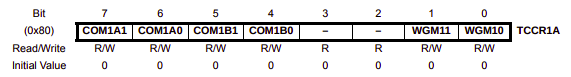
\includegraphics[width=\linewidth]{regA.png}}
\caption{Регістр TCCR1A.}
\label{fig:regA}
\end{figure}
\begin{figure}[h]
\center{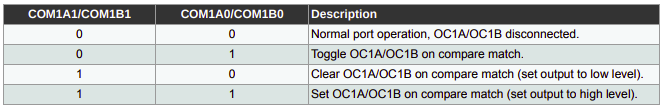
\includegraphics[width=\linewidth]{outputSet.png}}
\caption{Режими роботи виходів OC1A та 0C1B.}
\label{fig:outputSet}
\end{figure}
\begin{figure}[h]
\center{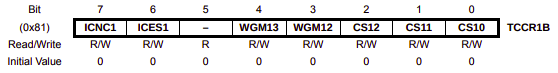
\includegraphics[width=\linewidth]{regB.png}}
\caption{Регістр TCCR1B.}
\label{fig:outputSet}
\end{figure}
\begin{figure}[h]
\center{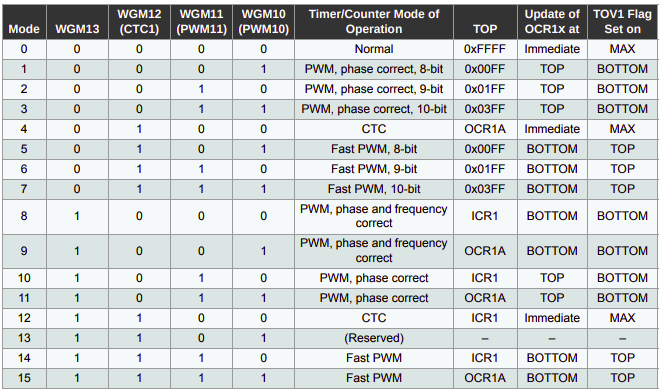
\includegraphics[width=\linewidth]{waveform.png}}
\caption{Різноманітні налаштування форми сигналів на виході.}
\label{fig:waveform}
\end{figure}
\begin{figure}[h]
\center{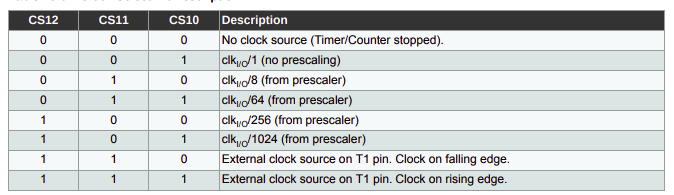
\includegraphics[width=\linewidth]{timermode.png}}
\caption{Доступні режими використання таймером тактового генератору.}
\label{fig:prescaler}
\end{figure}
Розглянемо регістр TCCR1A (Рис. \ref{fig:regA}). Біти 7-6 відповідають за режим роботи каналу А (ножка 0С1А, на Arduino Uno - D9), 5-4 - режим каналу Б (0С1В). Для нашої задачі, необхідно просто періодично подавати високу напругу на вихід Тому використовується режим порівняння на каналі А. Канал Б не задіяний. Всі режими роботи каналів показані на рис. \ref{fig:outputSet}

Таймер може видавати як звичайний так і різноманітний ШИМ сигнал. Але очевидно, що ці всі витребеньки нам не потрібні, тому в даній роботі використовується звичайний СТС режим, який передбачає очистку таймера при співпадінні його значення з деяким, наперед заданим. Тобто, використовується режим 4 на рис. \ref{fig:waveform}. Як видно із колонки TOP - значення, з яким буде порівнюватися таймер задається байтом 0СR1A.

Останні біти, потрібні нам (CS12 - CS10), відповідають за режим роботи самого таймеру. А саме, режим використання тактового генератору. Ми можемо використовувати частоту останнього 'як є', а можемо ділити її на різні степені двійки. Тобто використовувати так званий дільник, що буде уповільнувати роботу. Очевидно, що для наших цілей, такі речі можуть бути смертельними, тому в роботі зануляються всі біти, окрім CS10, тобто використовується режим без дільника (рис. \ref{fig:prescaler})
